Tübingen hat keine Universität, Tübingen \textbf{ist} eine Universität, daher
existiert auch kein Uni-Campus im herkömmlichen Sinne. Alles spielt sich
irgendwo in der Stadt ab, für euch im ersten Semester vor allem auf der
Morgenstelle, später auch auf dem Sand und der MvL. Damit ihr euch dort
zurechtfindet, haben wir hier ein paar Lagepläne zusammengefasst. Diese sind
keinesfalls allumfassend, sie sollen euch lediglich eine grobe Orientierung
durch den Dschungel der Uni-Gebäude bieten.

\begin{figure}[ht!]
	\begin{minipage}[t]{.5\linewidth}
		\centering
		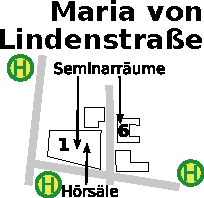
\includegraphics[width=0.6\linewidth]{shared/anhang/lageplaene/uebersicht_mvl.pdf}
	\end{minipage}%
	\begin{minipage}[t]{.5\linewidth}
		\centering
		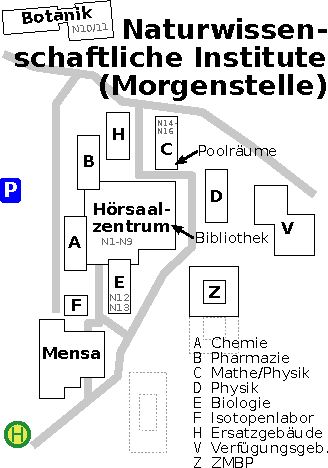
\includegraphics[width=0.9\linewidth]{shared/anhang/lageplaene/uebersicht_morgenstelle.pdf}
	\end{minipage}
\end{figure}

\begin{figure}[ht!]
	\centering
	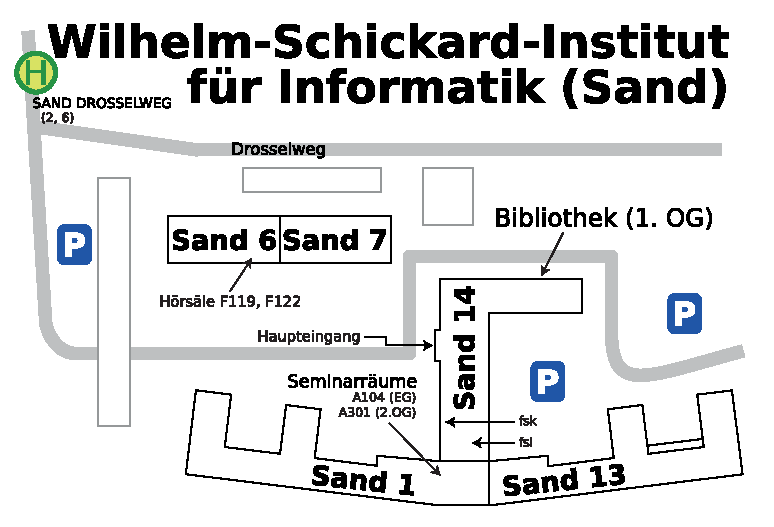
\includegraphics[width=0.6\textwidth]{shared/anhang/lageplaene/uebersicht_sand.pdf}
\end{figure}
%\subsubsection*{Sand, Erdgeschoss}~
%\begin{figure}[ht!]
%	\centering
%	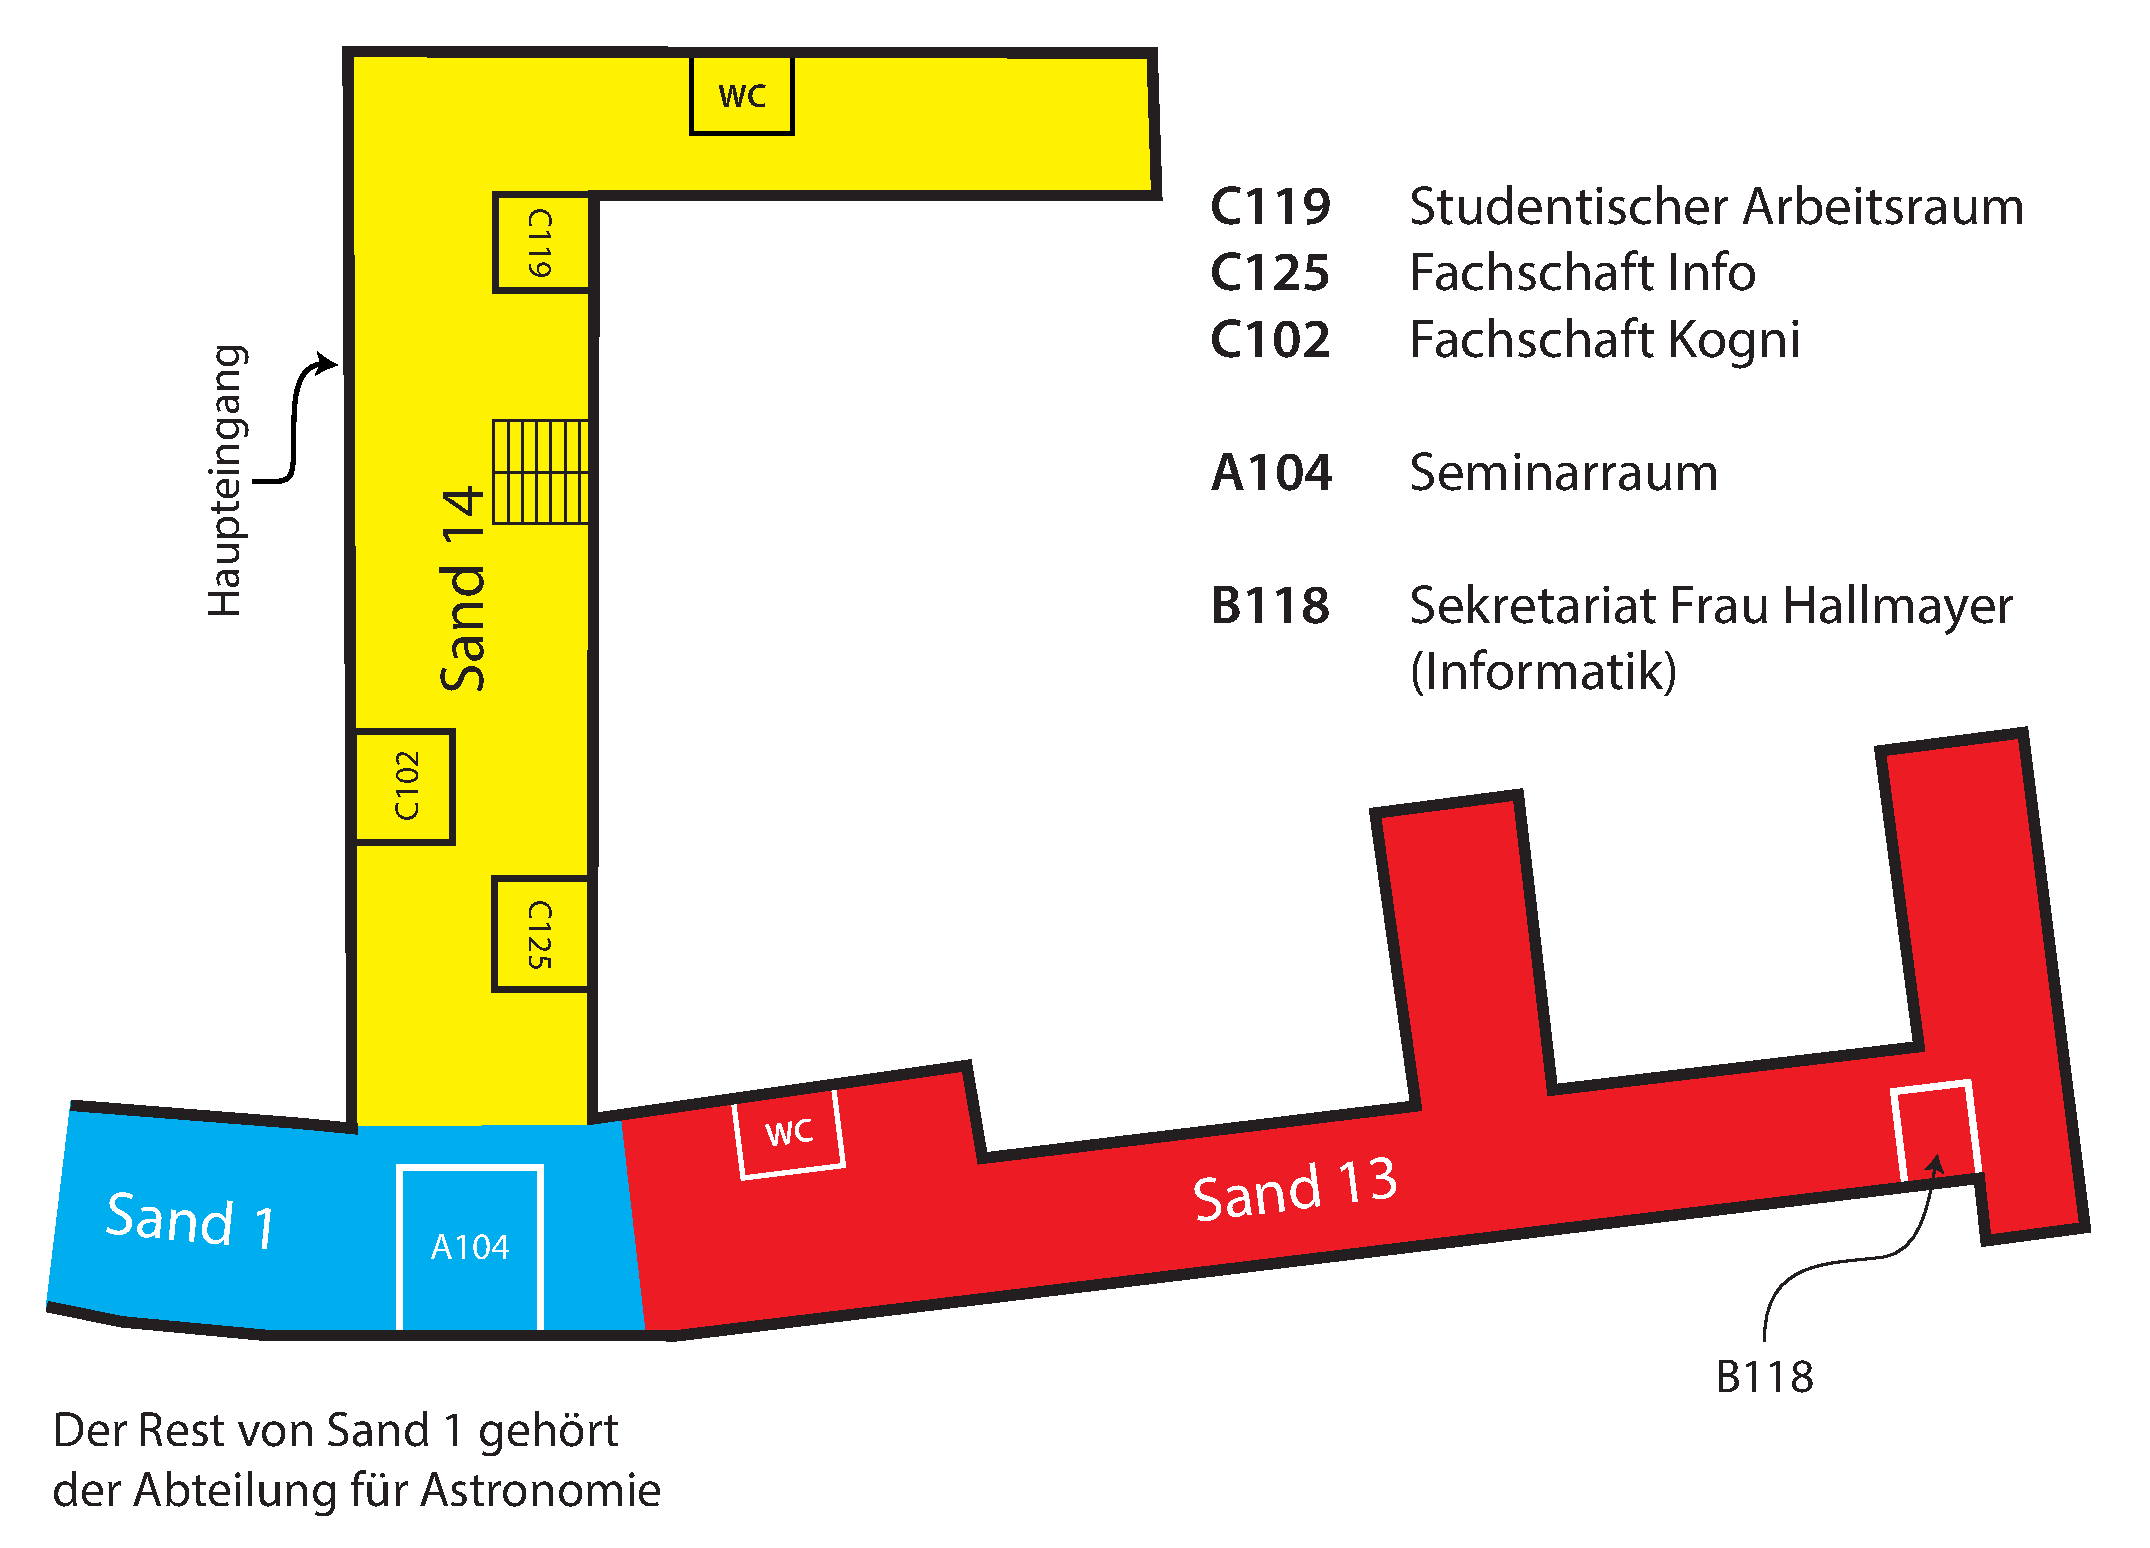
\includegraphics[width=0.9\textwidth]{shared/anhang/lageplaene/sand_eg.pdf}
%\end{figure}
%\vfill 
%\subsubsection*{Sand, 1. OG}~
%\begin{figure}[ht!]
%	\centering
%	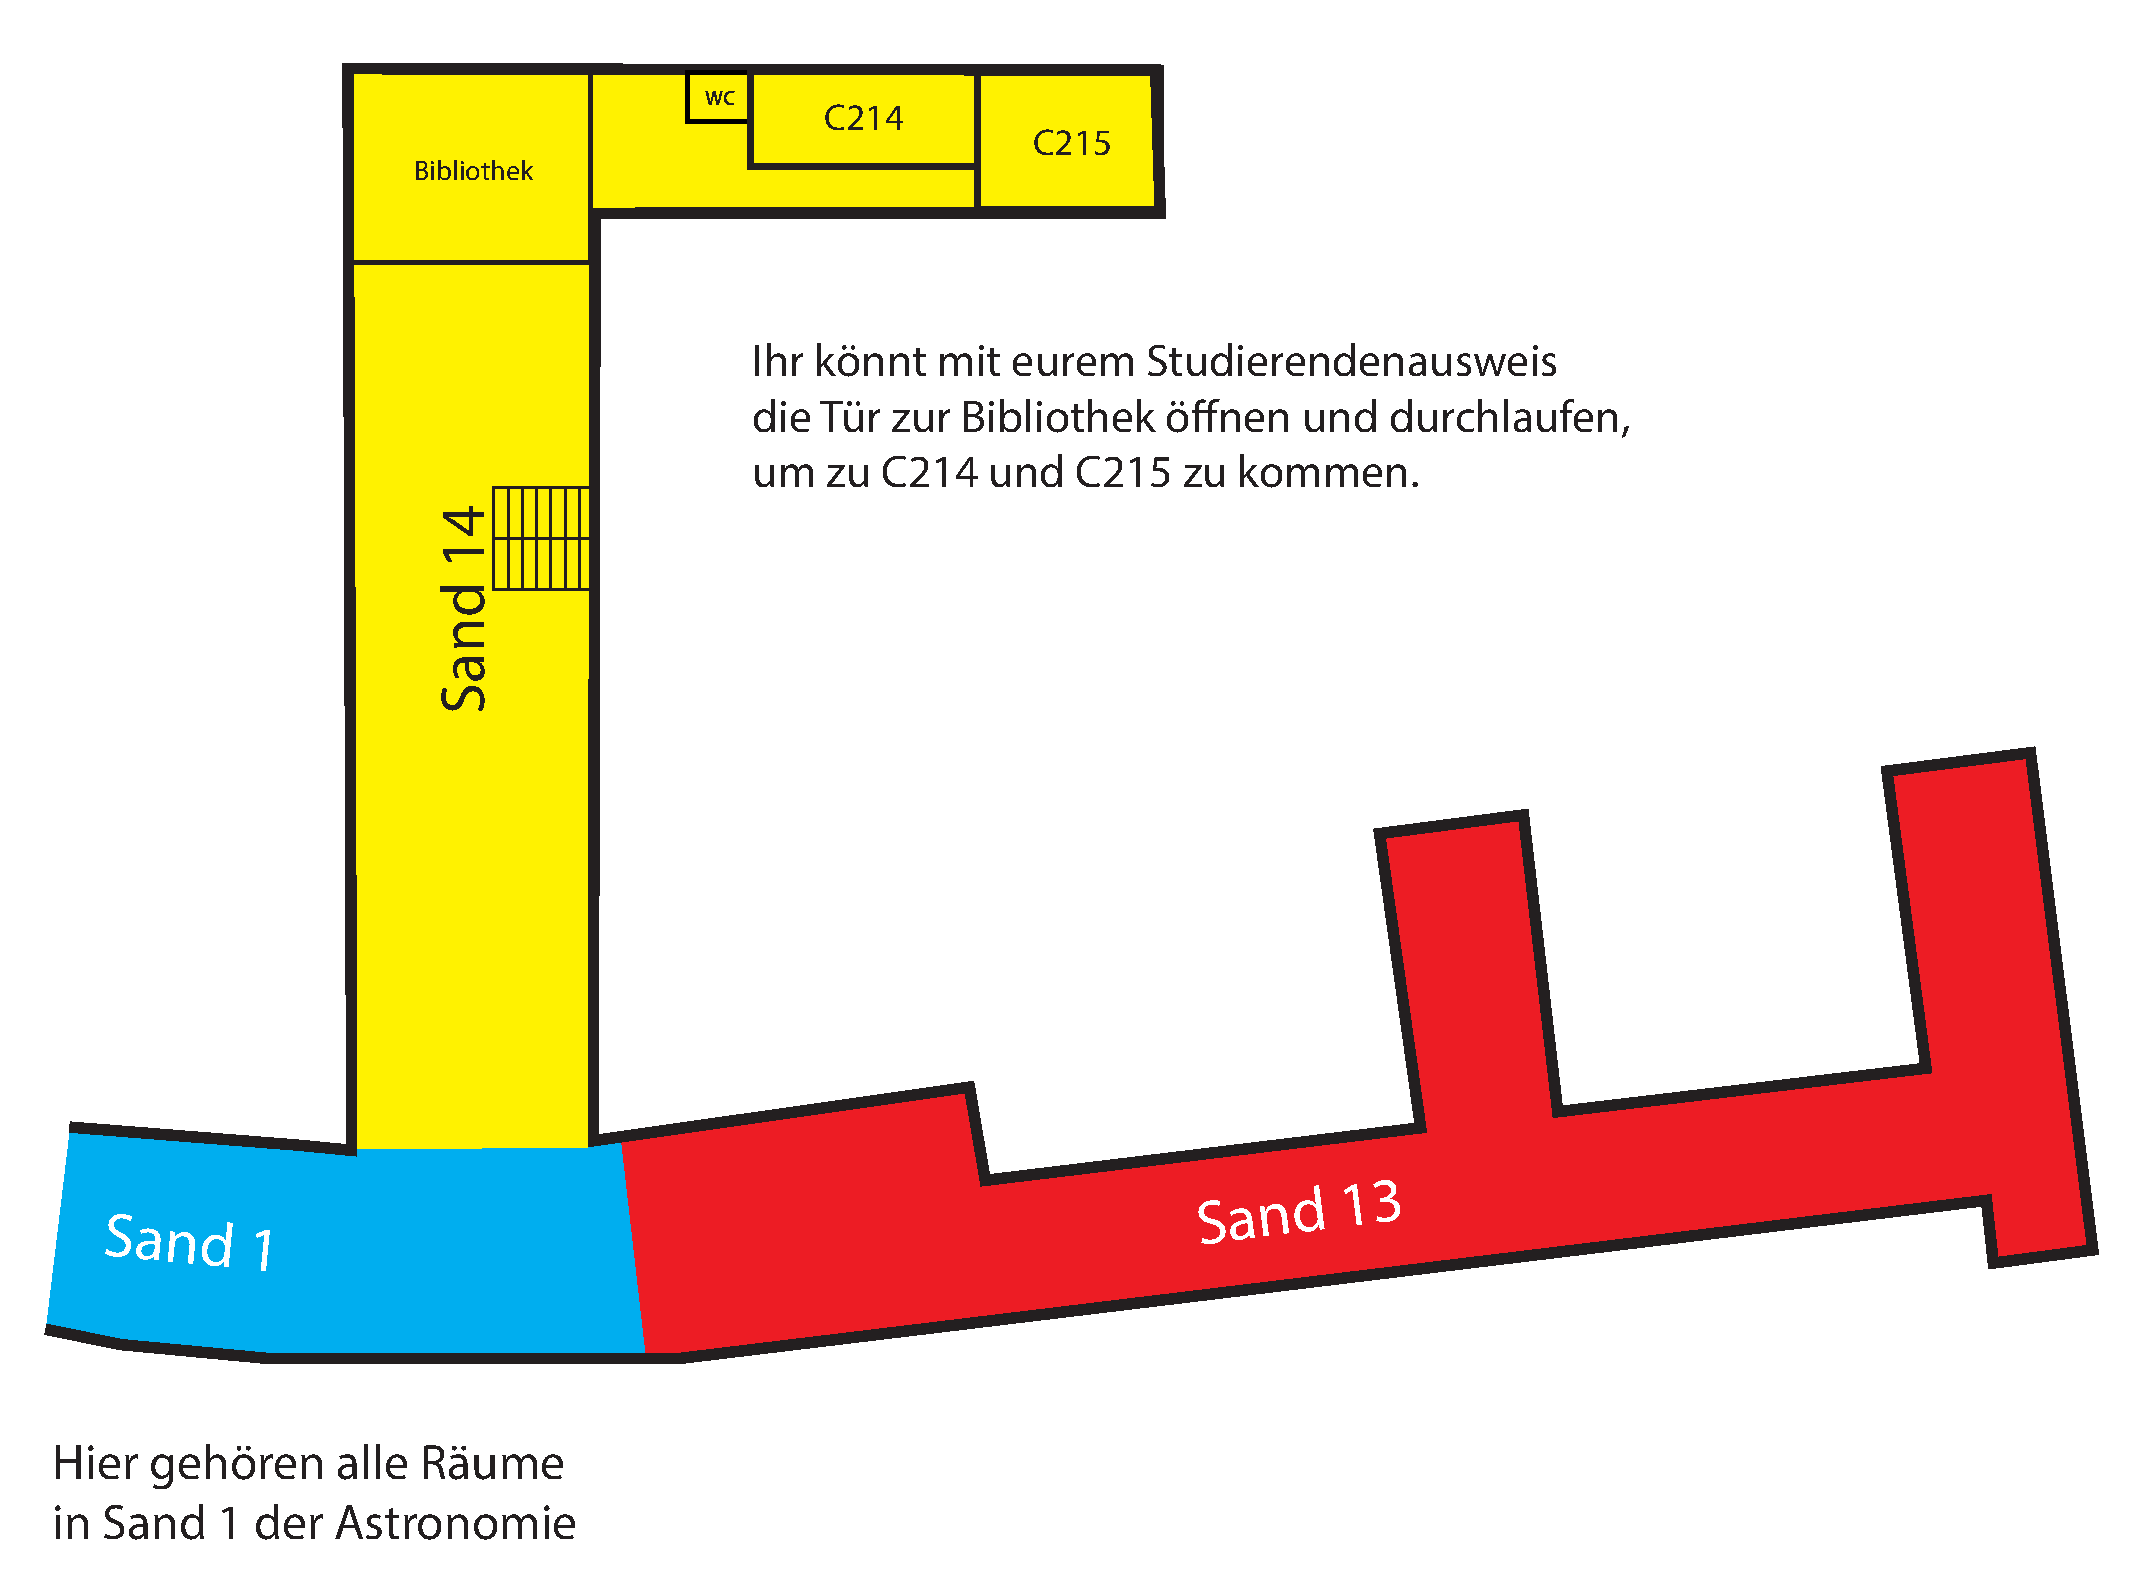
\includegraphics[width=0.9\textwidth]{shared/anhang/lageplaene/sand_1og.pdf}
%\end{figure}
%\subsubsection*{Sand, 2. OG}~
%\begin{figure}[ht!]
%	\centering
%	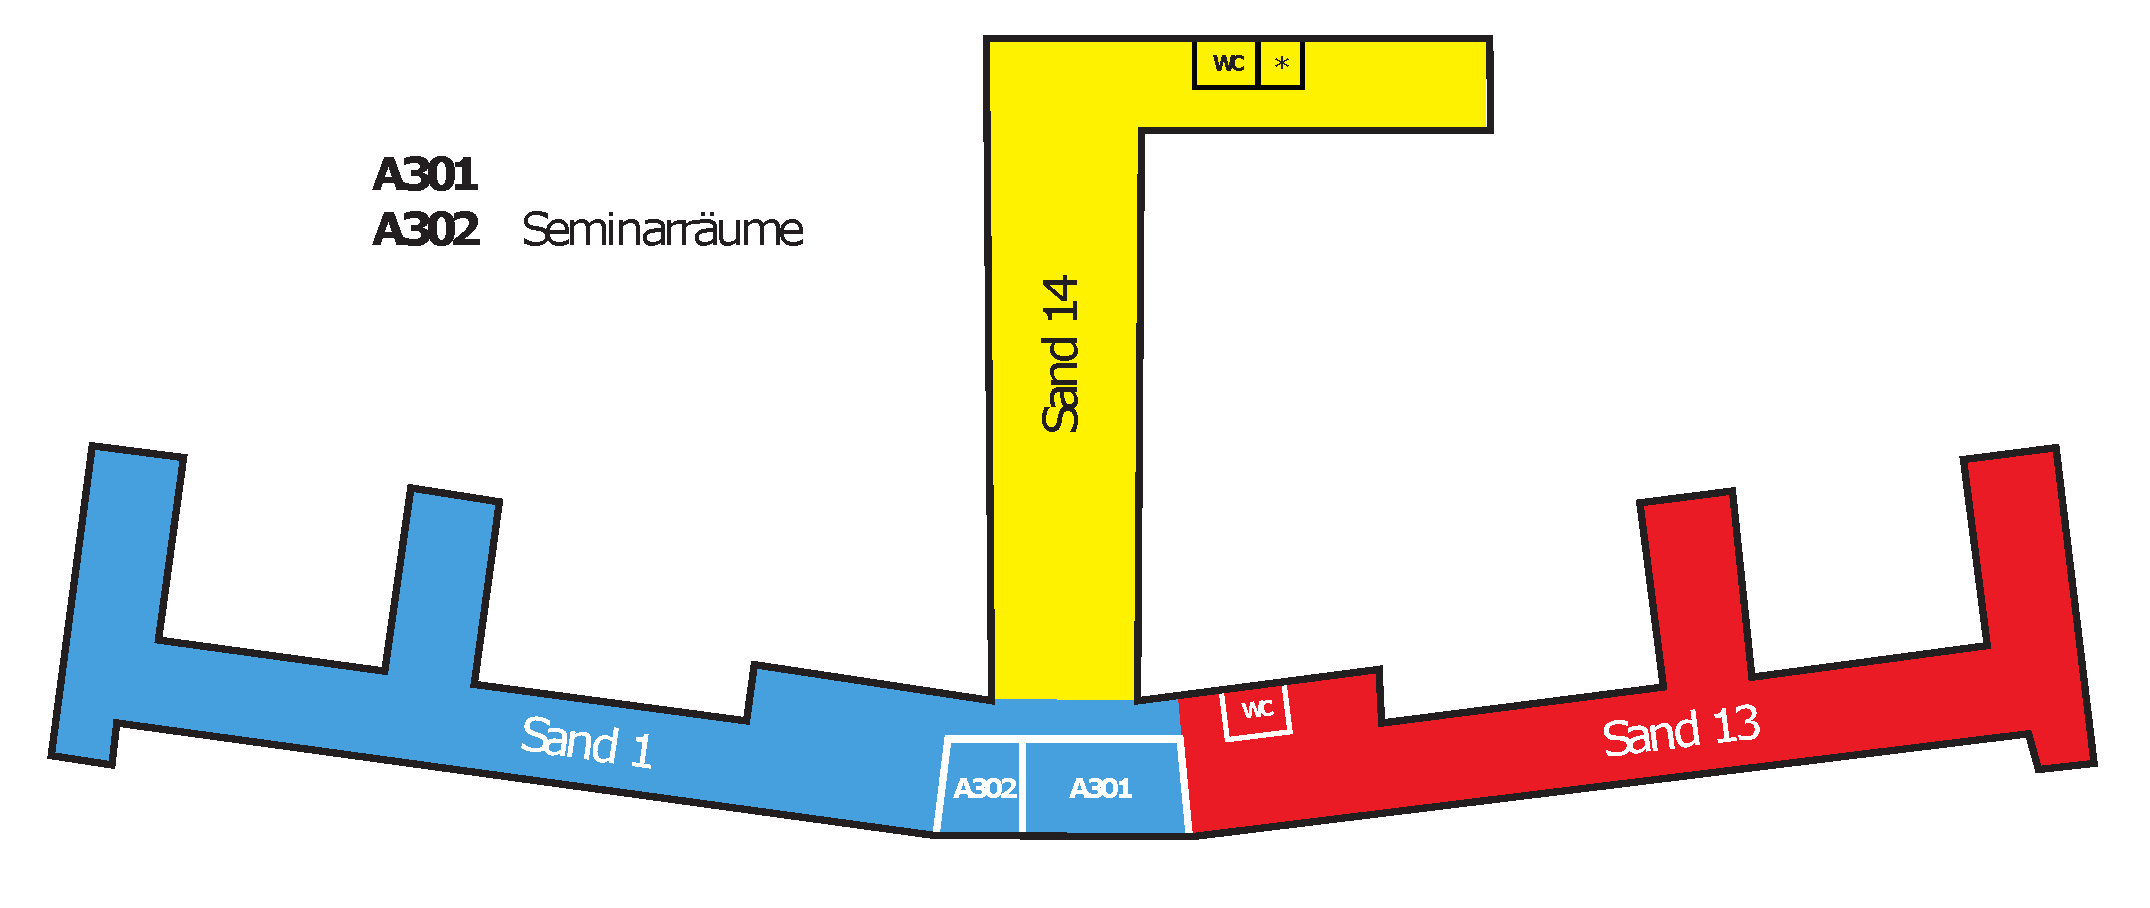
\includegraphics[width=\textwidth]{shared/anhang/lageplaene/sand_2og.pdf}
%\end{figure}
